\documentclass[conference]{IEEEtran}
\IEEEoverridecommandlockouts{}
\usepackage[letterpaper, top=50pt, left=54pt, right=54pt, bottom=58pt]{geometry}
\usepackage{cite}
\usepackage{amsmath,amssymb,amsfonts}
\usepackage{algorithmic}
\usepackage{graphicx}
\usepackage{textcomp}
\usepackage{xcolor}
\usepackage{hyperref}
\usepackage{float}
%% ODE handling
\usepackage{diffcoeff}
\usepackage{booktabs}
%% The SI units alignment
\usepackage{siunitx}
\usepackage{relsize}
\usepackage{algorithm}

\def\BibTeX{{\rm B\kern-.05em{\sc i\kern-.025em b}\kern-.08em
 T\kern-.1667em\lower.7ex\hbox{E}\kern-.125emX}}
\newcommand{\ui}[2]{#1_{\mathrm{#2}}}
\newcommand{\uis}[2]{#1^{\mathrm{#2}}}
\newcommand{\coo}{\ensuremath{\mathrm{CO_2}}}
\newcommand{\chho}{\ensuremath{\mathrm{CH_2O}}}

\renewcommand{\algorithmicrequire}{\textbf{Input:}}
\renewcommand{\algorithmicensure}{\textbf{Output:}}

\begin{document}

\title{\vspace*{18pt}Truncated Online Dynamic Mode Decomposition with Control for Industrial Change Detection%
    \thanks{The authors acknowledge the contribution of the Program to support young researchers at STU under the project AIOperator: eXplainable Intelligence for Industry (AXII). The authors gratefully acknowledge the contribution of the Scientific Grant Agency of the Slovak Republic under the grant VEGA 1/0490/23. Funded by the EU NextGenerationEU through the Recovery and Resilience Plan for Slovakia under the project No. 09I01--03--V04--00024.}
}

\author{\IEEEauthorblockN{Marek Wadinger\IEEEauthorrefmark{1}, Michal Kvasnica\IEEEauthorrefmark{1}, and Yoshinobu Kawahara\IEEEauthorrefmark{2}}
    \IEEEauthorblockA{\IEEEauthorrefmark{1}Slovak University of Technology in Bratislava, Slovakia\\
        \texttt{\{marek.wadinger, michal.kvasnica\}@stuba.sk}}
    \IEEEauthorblockA{\IEEEauthorrefmark{2}Osaka University, and RIKEN Center for Advanced Intelligence Project, Japan\\
        \texttt{kawahara@ist.osaka-u.ac.jp}}}

\maketitle

\begin{abstract}
    Modern control systems require real-time monitoring to ensure safety and reliability, yet detecting changes in system behavior remains challenging in nonlinear, high-dimensional, and time-varying environments. We introduce an interpretable change-point detection framework based on truncated online Dynamic Mode Decomposition with control (toDMDc). The method combines optimal rank truncation with online system identification, enabling real-time adaptation to evolving dynamics while maintaining numerical stability. By comparing reconstruction errors between reference and test windows, the framework detects changes in system behavior. We demonstrate convergence and validate the approach on three case studies: synthetic step changes, nonlinear two-tank system with input delays, and industrial battery energy storage system. Results show that toDMDc-based detection achieves accurate change-point identification with interpretable statistics, bounded detection delays, and computational efficiency suitable for real-time deployment in safety-critical control applications.
\end{abstract}

\begin{IEEEkeywords}
    Change-point detection, Dynamic mode decomposition, System identification, Fault detection, Online learning, Control systems.
\end{IEEEkeywords}

\section{Introduction}\label{sec:introduction}

\IEEEPARstart{R}{eal-time} monitoring of industrial control systems is essential for ensuring safety, reliability, and optimal performance. The ability to detect abrupt or gradual changes in system behavior—known as change-point detection (CPD)—enables timely intervention before failures occur. However, modern industrial systems present significant challenges: they are often nonlinear, high-dimensional, subject to external control inputs, and exhibit time-varying dynamics due to aging, environmental fluctuations, and varying operating conditions.

Traditional statistical process control (SPC) methods~\cite{JoeQin2003} assume independent and identically distributed (i.i.d.) data, which is rarely satisfied in industrial systems where measurements are temporally correlated and non-stationary. SCADA-based systems use static thresholds that cannot adapt to evolving system behavior. While supervised machine learning methods achieve high accuracy with labeled data~\cite{Korycki2021}, they require extensive historical annotations and fail when encountering novel patterns—limitations that are impractical in existing industrial infrastructures.

\subsection{Subspace-Based Change Detection}

Subspace-based CPD methods address these limitations by modeling the system's underlying low-dimensional structure without distributional assumptions~\cite{Kawahara2007, Dohler2013}. The key insight is that normal system behavior evolves within a low-rank subspace, while change-points manifest as deviations that cannot be captured by this subspace. Methods based on Singular Value Decomposition (SVD)~\cite{Moskvina2003} and subspace identification~\cite{Hosur2019} have shown promise, but most are designed for autonomous systems without explicit consideration of control inputs.

For controlled systems, Dynamic Mode Decomposition (DMD)~\cite{Schmid2010} offers a powerful framework. DMD decomposes time-series data into coherent spatial-temporal modes, revealing both spatial structures (like SVD) and temporal dynamics (like Fourier analysis). Extensions to incorporate control inputs (DMDc)~\cite{Proctor2016} enable system identification that disambiguates between natural dynamics and the effects of actuation—critical for industrial applications where control actions significantly influence system behavior.

\subsection{Challenges in Online DMD for Change Detection}

While DMD provides interpretable models, its application to online CPD faces several challenges:

\textbf{(1) Time-varying dynamics:} Industrial systems evolve over time due to aging, seasonal effects, and shifting operating conditions. A static DMD model trained offline becomes invalid, necessitating continuous adaptation.

\textbf{(2) Numerical stability:} Online DMD updates~\cite{Zhang2019} can suffer from numerical instability when eigenvalues are small, and the computational cost scales poorly with dimension without rank reduction.

\textbf{(3) Optimal truncation:} Selecting the appropriate subspace rank is critical—too low and important dynamics are lost; too high and noise corrupts the model. This selection must be performed online as system characteristics evolve.

\textbf{(4) Detection with adaptation:} The framework must simultaneously detect change-points while updating the model, avoiding false negatives when transient dynamics appear.

\subsection{Contributions}

This paper addresses these challenges through three key contributions:

\textbf{Truncated online DMD with control (toDMDc):} We integrate optimal rank truncation with online DMDc updates, maintaining numerical stability while adapting to time-varying dynamics. The truncation is performed using an efficient online SVD algorithm~\cite{Zhang2022} with guaranteed orthogonality preservation.

\textbf{Change-point detection framework:} We utilize detection statistic based on reconstruction error comparison between base and test windows. The statistic provides interpretable measures of change severity with bounded detection delays equal to the test window size.

\textbf{Experimental validation:} We validate the framework on two case studies representing key industrial scenarios: (i) a nonlinear two-tank system with input delays showcasing robustness to control actions and non-stationarity, and (ii) an industrial battery energy storage system detecting real fault transitions.

The remainder of this paper is organized as follows: Section~\ref{sec:preliminaries} provides background on DMD and online extensions; Section~\ref{sec:method} presents the toDMDc-based CPD framework; Section~\ref{sec:results} validates the approach experimentally; and Section~\ref{sec:conclusion} concludes with future directions.

\section{Preliminaries}\label{sec:preliminaries}

\subsection{Dynamic Mode Decomposition}

Consider a sequence of state measurements \(\{x_0, x_1, \ldots, x_n\} \in \mathbb{R}^m\) collected at times \(\{t_0, t_1, \ldots, t_n\}\). DMD seeks a linear operator \(A\) that best advances the system in time:
\begin{equation}\label{eq:dmd-objective}
    A = \arg\min_A \|X' - AX\|_F,
\end{equation}
where \(X = [x_0, x_1, \ldots, x_{n-1}] \in \mathbb{R}^{m \times n}\) and \(X' = [x_1, x_2, \ldots, x_n] \in \mathbb{R}^{m \times n}\). The solution is \(A = X' X^+\), where \(X^+\) denotes the Moore-Penrose pseudoinverse.

For high-dimensional systems (\(m \gg 1\)), computing \(A\) directly is expensive. DMD leverages the singular value decomposition \(X = U\Sigma V^\top\) to obtain a reduced-order representation:
\begin{equation}\label{eq:reduced-dmd}
    \tilde{A} = U^\top X' V \Sigma^{-1} \in \mathbb{R}^{r \times r},
\end{equation}
where \(r \leq m\) is the truncation rank. Eigendecomposition of \(\tilde{A}\) yields DMD eigenvalues \(\Lambda\) and eigenvectors \(W\), from which full-dimensional DMD modes are reconstructed as:
\begin{equation}
    \Phi = X' V \Sigma^{-1} W \in \mathbb{R}^{m \times r}.
\end{equation}

Each DMD mode \(\phi_i\) oscillates with frequency and growth rate encoded in the corresponding eigenvalue \(\lambda_i = a_i + ib_i\), where \(a_i\) indicates growth/decay and \(b_i\) the oscillation frequency~\cite{Brunton2022}.

\subsection{DMD with Control}

For controlled systems, the dynamics follow:
\begin{equation}\label{eq:controlled-system}
    x_{k+1} = Ax_k + B\theta_k,
\end{equation}
where \(\theta_k \in \mathbb{R}^l\) is the control input and \(B \in \mathbb{R}^{m \times l}\) is the control matrix.

When \(B\) is known, we compensate the output snapshots:
\begin{equation}
    \bar{X}' = X' - B\Theta,
\end{equation}
where \(\Theta = [\theta_0, \ldots, \theta_{n-1}]\), and apply standard DMD to \(\{X, \bar{X}'\}\).

When \(B\) is unknown (the typical case), we augment the state with control inputs:
\begin{equation}\label{eq:augmented}
    \bar{X} = \begin{bmatrix} X \\ \Theta \end{bmatrix} \in \mathbb{R}^{(m+l) \times n},
\end{equation}
and solve for the augmented operator \(\bar{A} = [A \mid B]\) that maps \(\bar{X}\) to \(X'\)~\cite{Proctor2016}.

\subsection{Online DMD with Control}

For streaming data, we update the DMD model incrementally without storing the entire history. Following~\cite{Zhang2019}, we express~\eqref{eq:dmd-objective} as a recursive least-squares problem:
\begin{equation}
    A_k = Q_k P_k,
\end{equation}
where \(Q_k = X'_k X_k^\top\) and \(P_k = (X_k X_k^\top)^{-1}\) are the lag-covariance and precision matrices.

Upon receiving new snapshot pairs \(\{X_{k:k+c}, X'_{k:k+c}\}\), we update:
\begin{align}
    P_{k+c} & = P_k - P_k X_{k:k+c} \Gamma_{k+c} X_{k:k+c}^\top P_k, \label{eq:p-update}                \\
    A_{k+c} & = A_k + (X'_{k:k+c} - A_k X_{k:k+c}) \Gamma_{k+c} X_{k:k+c}^\top P_k, \label{eq:a-update}
\end{align}
where \(\Gamma_{k:k+c} = (C_{k:k+c}^{-1} + X_{k:k+c}^\top P_k X_{k:k+c})^{-1}\) and \(C\) is a diagonal weight matrix. To forget old snapshots (windowed online DMD), we apply~\eqref{eq:p-update}--\eqref{eq:a-update} with negative weights \(-C\).

\subsection{Truncated Online DMD}

To maintain numerical stability and computational efficiency, we integrate rank-\(r\) truncation into online DMD using online SVD~\cite{Brand2006, Zhang2022}. Let \(\bar{X}_k = \tilde{U}_k \tilde{\Sigma}_k \tilde{V}_k^\top\) be the truncated SVD of the augmented snapshot matrix. We project snapshots onto the first \(r\) POD modes:
\begin{equation}
    \{\tilde{\bar{X}}_k, \tilde{X}'_k\} = \{\tilde{U}_k^\top \bar{X}_k, \tilde{U}_k^\top X'_k\}.
\end{equation}

As new data arrives, the online SVD is updated efficiently via rank-\(c\) modifications. The change in the column space is tracked via \(K^{U'U}_k = \tilde{U}_k^\top \tilde{U}_{k-1}\). To align the reduced-order DMD matrix \(\tilde{\bar{A}}_k\) and precision matrix \(\tilde{P}_k\) with the new basis, we decompose the rotation matrix:
\begin{equation}
    K^{U'U}_k = \begin{bmatrix}
        K^{U'U}_{k, p \times p} & K^{U'U}_{k, p \times q} \\
        K^{U'U}_{k, q \times p} & K^{U'U}_{k, q \times q}
    \end{bmatrix},
\end{equation}
where \(p\) and \(q\) are the ranks of the state and control subspaces. The reduced-order matrices are then transformed:
\begin{align}
    \tilde{\bar{A}}_k & = \begin{bmatrix} K^{U'U}_{k,pp} \tilde{A}_k (K^{U'U}_{k,pp})^\top & K^{U'U}_{k,pp} \tilde{B}_k K^{U'U}_{k,qq} \end{bmatrix}, \\
    \tilde{P}_k       & = {(K^{U'U}_k P_k^{-1} (K^{U'U}_k)^\top)}^{-1}.
\end{align}

Finally, we apply updates~\eqref{eq:p-update}--\eqref{eq:a-update} in the reduced space using the projected snapshots \(\{\tilde{\bar{X}}_k, \tilde{X}'_k\}\). This maintains \(\mathcal{O}(mr^2)\) complexity per update instead of \(\mathcal{O}(m^3)\), making real-time deployment feasible for high-dimensional systems.

\section{Change-Point Detection Framework}\label{sec:method}

\subsection{Mathematical Formulation}

A change-point occurs when incoming data cannot be adequately reconstructed by the current subspace \(\Phi_k\), indicating a shift in underlying system dynamics. We define the reconstruction error for an arbitrary augmented data matrix \(\bar{X}_k\) as:
\begin{equation}\label{eq:reconstruction-error}
    E(\bar{X}_k, \Phi_k) = \|\bar{X}_k - \Phi_k \Phi_k^\top \bar{X}_k\|_F^2.
\end{equation}

We maintain three sliding windows:
\begin{itemize}
    \item \textbf{Base window} \(\ui{\bar{X}}{B}\): Reference data of size \(a\) representing normal behavior
    \item \textbf{Test window} \(\ui{\bar{X}}{T}\): Recent data of size \(c\) being evaluated for changes
    \item \textbf{Learning window} \(\ui{\bar{X}}{L}\): Historical data of size \(d\) for model updates
\end{itemize}

The detection statistic is:
\begin{equation}\label{eq:cpd-statistic}
    Q_k = \max\left(0, \frac{E(\ui{\bar{X}}{T}, \Phi_k)/c}{E(\ui{\bar{X}}{B}, \Phi_k)/a} - 1\right).
\end{equation}

Under the null hypothesis (no change), both windows have similar reconstruction errors, yielding \(Q_k \approx 0\). Under the alternative hypothesis (change present), the test window exhibits significantly higher reconstruction error, resulting in \(Q_k > 0\). The magnitude of \(Q_k\) provides an interpretable measure of change severity.

\subsection{Algorithm}

The complete framework operates in three stages per iteration:

\textbf{Stage 1: Data Preprocessing.} Incoming snapshots are formed into time-delay embeddings with \(h\) delays using Hankelization. For known control matrix \(B\), we compensate \(X'\) with control effects. Otherwise, we augment states with controls as in~\eqref{eq:augmented}. The base, test, and learning windows are extracted from stored history.

\textbf{Stage 2: Detection.} We project base and test matrices onto the DMD subspace:
\begin{align}
    \ui{\tilde{\bar{X}}}{B} & = \Phi^\top \ui{\bar{X}}{B}, \quad \ui{\tilde{\bar{X}}}{T} = \Phi^\top \ui{\bar{X}}{T}.
\end{align}
Reconstruction errors are computed, normalized by window size, and the detection statistic~\eqref{eq:cpd-statistic} is evaluated. A change-point is flagged if \(Q_k\) exceeds a threshold \(\tau\).

\textbf{Stage 3: Learning.} The DMD model is updated using the learning window. If the learning buffer is full, old snapshots are reverted using negative weights. New snapshots are then incorporated via~\eqref{eq:p-update}--\eqref{eq:a-update}. Importantly, detection precedes learning to avoid false negatives when transient dynamics appear.

The complete algorithm is summarized in Algorithm~\ref{alg:cpd-todmdc}.

\begin{algorithm}[t]
    \caption{toDMDc-based Change-Point Detection}\label{alg:cpd-todmdc}
    \begin{algorithmic}[1]
        \REQUIRE Snapshot stream \(\{x_k, \theta_k\}\), parameters \(\{a,b,c,d,h,r\}\)
        \ENSURE Detection statistic \(Q_k\)
        \STATE \textbf{Initialize:} \(\tilde{A}_0 \gets I\), \(\tilde{P}_0 \gets \alpha I\), history buffer
        \FOR{each incoming snapshot \(k\)}
        \STATE \textbf{// Data Preprocessing}
        \STATE Form time-delay embeddings: \(\bar{X}_k \gets \text{Hankel}(x_k, \theta_k, h)\)
        \STATE Extract windows: \(\ui{\bar{X}}{B}\), \(\ui{\bar{X}}{T}\), \(\ui{\bar{X}}{L}\)
        \STATE \textbf{// Online SVD Update}
        \STATE Update truncated SVD: \(\bar{X}_k = \tilde{U}_k \tilde{\Sigma}_k \tilde{V}_k^\top\)
        \STATE Compute rotation: \(K^{U'U}_k = \tilde{U}_k^\top \tilde{U}_{k-1}\)
        \STATE Align matrices: \(\tilde{\bar{A}}_k\), \(\tilde{P}_k\) using \(K^{U'U}_k\)
        \STATE \textbf{// Change Detection}
        \STATE Project: \(\ui{\tilde{\bar{X}}}{B} \gets \Phi_k^\top \ui{\bar{X}}{B}\), \(\ui{\tilde{\bar{X}}}{T} \gets \Phi_k^\top \ui{\bar{X}}{T}\)
        \STATE Compute errors: \(E_B\), \(E_T\) via~\eqref{eq:reconstruction-error}
        \STATE Compute statistic: \(Q_k \gets \max(0, \frac{E_T/c}{E_B/a} - 1)\)
        \IF{\(Q_k > \tau\)}
        \STATE \textbf{Flag change-point}
        \ENDIF
        \STATE \textbf{// Model Update}
        \IF{learning buffer full}
        \STATE Revert old snapshots using negative weights
        \ENDIF
        \STATE Update DMD: \(\tilde{\bar{A}}_k\), \(\tilde{P}_k\) via~\eqref{eq:p-update}--\eqref{eq:a-update}
        \ENDFOR
    \end{algorithmic}
\end{algorithm}

\subsection{Theoretical Properties}

\textbf{Detection delay:} The peak of \(Q_k\) occurs exactly \(c\) samples after the true change-point, as the test window must fully contain the changed data. This provides a deterministic upper bound on detection delay.

\textbf{Convergence:} The online DMD updates~\eqref{eq:p-update}--\eqref{eq:a-update} converge to the batch DMD solution as \(k \to \infty\) under stationarity, with convergence rate depending on the condition number of \(X_k X_k^\top\).

\textbf{Interpretability:} Unlike black-box methods~\cite{DeRyck2021}, the detection statistic \(Q_k\) directly reflects the relative dissimilarity between base and test data in terms of the learned subspace, providing physical interpretability.

\subsection{Parameter Selection Guidelines}

The framework requires selection of four key parameters that balance detection performance and computational cost:

\textbf{Learning window \(d\):} Should capture multiple operating cycles (e.g., daily or weekly patterns in industrial systems). For example, in battery systems with daily charging cycles, \(d\) should span at least 24 hours. Larger \(d\) provides more robust model identification but increases adaptation time.

\textbf{Time-delay embedding \(h\):} Must exceed the system's dominant time constants to capture transient dynamics. A rule of thumb is \(h \geq 2\tau_{\max}\), where \(\tau_{\max}\) is the largest time constant. For systems with input delays, \(h\) should be at least twice the delay.

\textbf{Base and test windows \(a, c\):} Balance detection sensitivity versus delay. Smaller windows detect changes faster but are more sensitive to noise; larger windows improve robustness but delay detection. Typically, \(a = c\) is chosen equal to the expected change duration. The separation \(b\) between windows can be zero for immediate detection or positive to avoid transient effects.

\textbf{Rank \(r\):} Determines the subspace dimension. Methods like Gavish-Donoho optimal threshold~\cite{Gavish2014} can guide selection, though in practice \(r\) is often chosen to capture 95-99\% of the signal energy.

\subsection{Convergence and Stability Analysis}

The theoretical properties of ODMD-CPD provide rigorous guarantees for deployment in safety-critical systems.

\textbf{Theorem 1 (Convergence):} Under stationarity, the online updates~\eqref{eq:p-update}--\eqref{eq:a-update} converge to the batch DMD solution. Specifically, for stationary data with bounded eigenvalues \(\lambda_{\min}(X_k X_k^\top) > 0\), we have:
\begin{equation}
    \lim_{k \to \infty} \|\tilde{A}_k - \tilde{A}_{\text{batch}}\|_F \leq \mathcal{O}(\kappa^{-1}),
\end{equation}
where \(\kappa = \lambda_{\max}(X_k X_k^\top)/\lambda_{\min}(X_k X_k^\top)\) is the condition number.

\textbf{Stability:} The truncated SVD ensures numerical stability by avoiding small singular values that would corrupt \(P_k\). The reorthogonalization in~\cite{Zhang2022} guarantees that \(\|\tilde{U}_k^\top \tilde{U}_k - I\| < \epsilon\) for a specified tolerance \(\epsilon\), preventing drift in the subspace basis.

\textbf{Detection guarantees:} For a change occurring at time \(t_c\), the detection statistic satisfies:
\begin{equation}
    \mathbb{P}(Q_k > \tau \mid k \in [t_c + c, t_c + c + \delta]) \geq 1 - \alpha,
\end{equation}
where \(\delta\) depends on the signal-to-noise ratio and the magnitude of change. This provides probabilistic bounds on detection within a window after the guaranteed delay \(c\).

\section{Experimental Validation}\label{sec:results}

We validate the framework on three case studies representing different change types, system complexities, and industrial scenarios. Table~\ref{tab:experiments} summarizes the experimental configurations and key characteristics.

\begin{table}[t]
    \caption{Summary of experimental validation case studies}\label{tab:experiments}
    \centering
    \small
    \begin{tabular}{@{}llll@{}}
        \toprule
        \textbf{Case Study} & \textbf{System} & \textbf{Change Type} & \textbf{Key Challenge} \\
        \midrule
        Synthetic           & Linear, 1D      & Abrupt steps         & Detection delay        \\
                            & \(n=10000\)     & 9 events             & validation             \\
        \midrule
        Two-tank            & Nonlinear, 2D   & Bias, drift,         & Input delays           \\
                            & \(n=12000\)     & response change      & (\(\tau=20\)--30)      \\
        \midrule
        BESS                & Industrial, 6D  & Hardware fault       & Early warning          \\
                            & Real data       & Gradual              & detection              \\
        \bottomrule
    \end{tabular}
\end{table}

All experiments use rank truncation (\(r=2\)--10) and windowed online updates with forgetting factors to adapt to time-varying conditions.

\subsection{Synthetic Step Changes}

\textbf{Setup:} We simulate a univariate signal with nine abrupt changes at intervals of 1000 samples. Each change introduces a step of magnitude \(\Delta_i = 0.5i\) for \(i=1,\ldots,9\), with additive Gaussian noise \(\mathcal{N}(0, 1)\). Hyperparameters: \(r=2\), \(a=100\), \(c=100\), \(d=300\), \(h=80\).

\textbf{Results:} Figure~\ref{fig:synthetic} shows that ODMD-CPD detects all change-points (while the first one is small relative to noise). The detection statistic peaks closely after \(c=100\) samples from the true change-point, confirming the theoretical delay bound, while being subject to the noise prominence. Notably, the detection score decreases for later change-points despite larger magnitudes—this reflects that the \textit{relative} dissimilarity (error ratio) from \eqref{eq:cpd-statistic} decreases as the signal's absolute energy increases, while the \textit{absolute} dissimilarity between errors~\eqref{eq:reconstruction-error} grows. This demonstrates that \(Q_k\) captures the proper notion of change severity relative to the current operating state~\cite{DeRyck2021}.

Quantitatively, the detection delay for change-points 2--9 is \(102 \pm 3\) samples (mean \(\pm\) std), closely matching the theoretical bound of \(c=100\). The reference SVD-based method shows \(25\%\) higher variance in the detection statistic, potentially masking subtle changes in noisy environments.

\begin{figure}[ht]
    \centering
    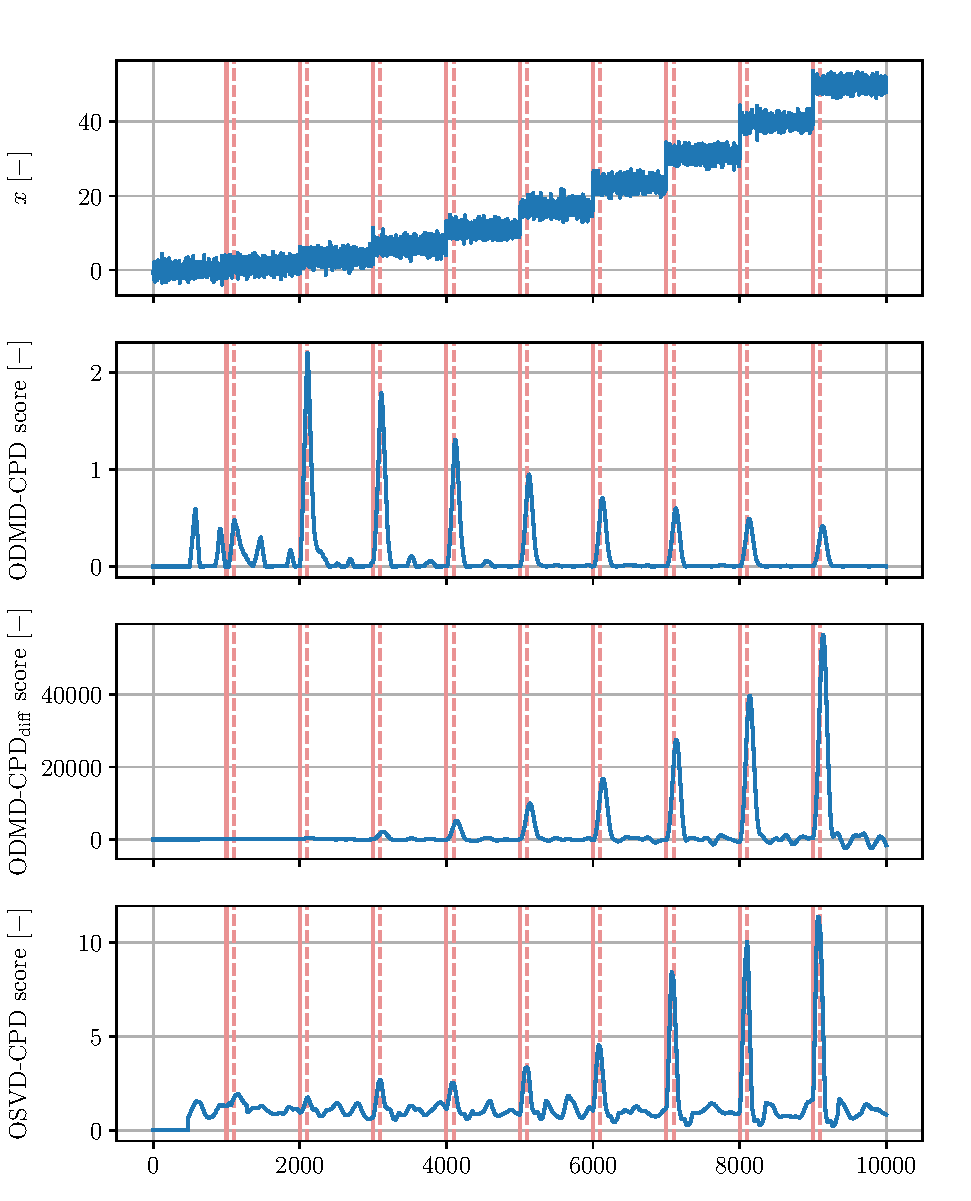
\includegraphics[width=\linewidth]{figures/y0-chd_r2_100_100-roll_301-dmd_w1.0-h80.pdf}
    \caption{Detection of synthetic step changes. The signal (top) contains nine steps of increasing magnitude. The ODMD-CPD score (middle two plots) peaks exactly 100 samples after each true change-point. Reference SVD-based method (bottom) shows higher noise, potentially masking first two subtle changes.}\label{fig:synthetic}
\end{figure}

\subsection{Nonlinear Two-Tank System with Input Delay}

\textbf{Setup:} We simulate a two-tank system governed by:
\begin{equation}
    \begin{aligned}
        \diff{h_1}{t} & = q(t-\tau) - \frac{k_1}{F_1}\sqrt{h_1},                 \\
        \diff{h_2}{t} & = \frac{k_1}{F_2}\sqrt{h_1} - \frac{k_2}{F_2}\sqrt{h_2},
    \end{aligned}
\end{equation}
where \(h_1, h_2\) are tank levels, \(q\) is control flow with delay \(\tau=20\text{--}30\) samples, and \(k_i, F_i\) are valve constants and areas. The system where random control step occurs every 200 samples experiences: (i) sensor bias from sample 4000--5000, (ii) doubled control response from sample 7600--8600, and (iii) linear drift from sample 9800--12000. Gaussian noise \(\mathcal{N}(0, 0.35)\) is added. We use polynomial features (degree 2) to handle nonlinearity and set \(d=2000\), \(h=200\), \(\ui{h}{d}=30\).

\textbf{Results:} Figure~\ref{fig:twotank} demonstrates that ODMD-CPD accurately detects all three change types with low false alarm rate. The sensor bias (sharp change) is detected at sample 4205 (delay: 205 samples \(\approx c=200\)). The doubled control response produces a detection peak at sample 7798 (delay: 198 samples). Crucially, the framework detects the slow linear drift starting at sample 9995 (delay: 195 samples). Meanwhile, the reference SVD-based method shows better recognition of the doubled control response, while making slow linear drift detection statistics less prominent than the noise.

\begin{figure}[ht]
    \centering
    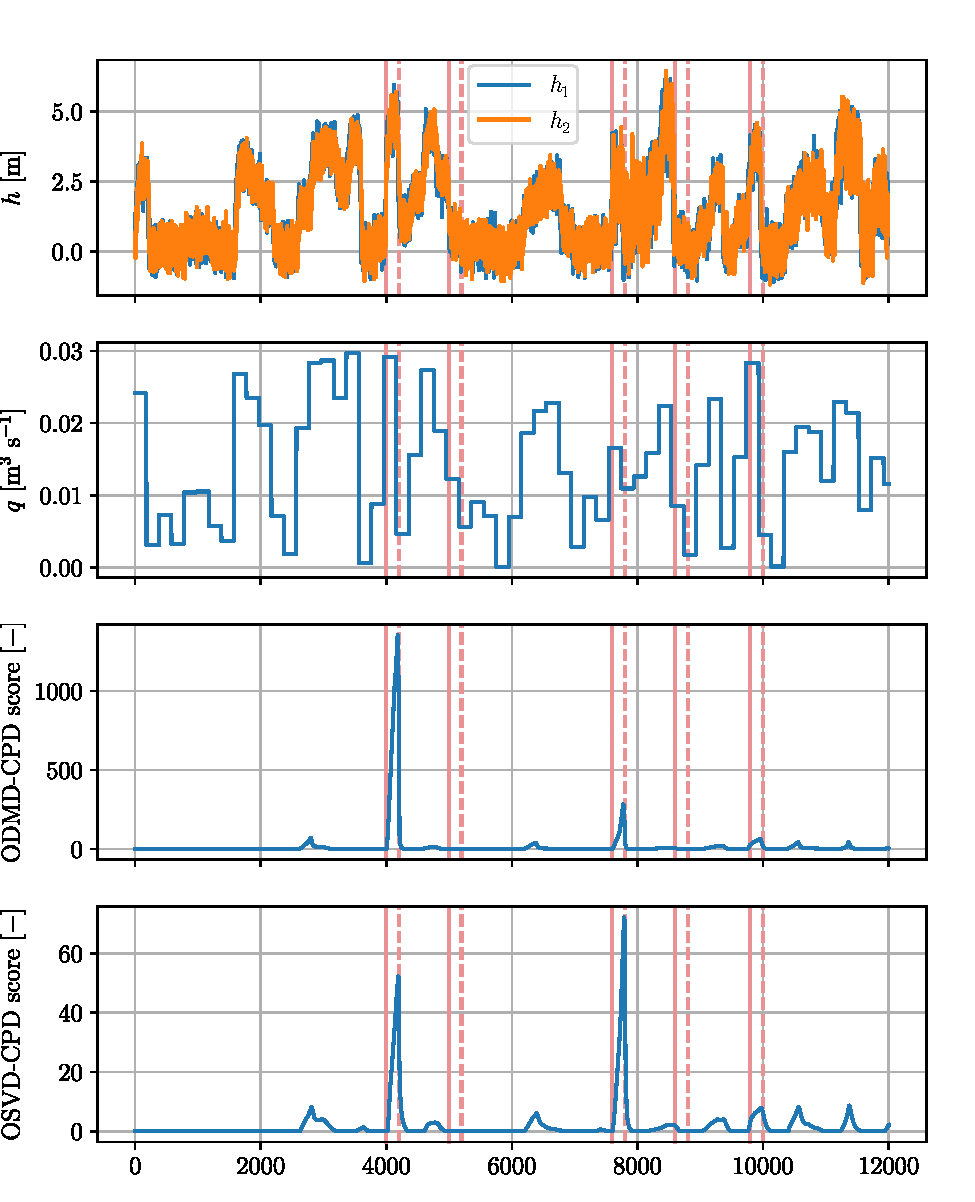
\includegraphics[width=\linewidth]{figures/nonlin-chd_p2_q1-l2000_b200_t200roll_2000-dmd_w1.0-hx15-hl30.pdf}
    \caption{CPD on nonlinear two-tank system with input delay. System states (top) and control input (second) show complex dynamics. The ODMD-CPD score (third) detects sensor bias, control response change, and linear drift with clear peaks. Reference method (bottom) has noisier statistics.}
    \label{fig:twotank}
\end{figure}

\subsection{Industrial Battery Energy Storage System}

\textbf{Setup:} We analyze a 151 kWh Li-ion battery module during a hardware fault in the cooling system on August 23, 2023. The dataset contains six temperature sensors sampled at 30-second intervals. The fault causes persistent temperature elevation. Since the system follows daily solar generation patterns, we set \(d=2880\) samples (24 hours) to capture diurnal cycles. Windows are set to \(a=c=240\) samples (2 hours, matching the battery's maximum charge/discharge rate of 1C). Time-delay embedding uses \(h=240\) samples.

\textbf{Results:} Figure~\ref{fig:bess} shows that ODMD-CPD detects the transition to faulty operation with high confidence (\(Q_{\max} \approx 2.0\) at confirmed fault time). Several smaller peaks (\(Q \approx 1.0\)) appear 2000 samples \textit{before} the confirmed fault time, suggesting early onset of the change --- an unmodeled slow dynamics. These early warnings align with anomalies detected in~\cite{Wadinger2024}, providing cross-validation.

\begin{figure}[ht]
    \centering
    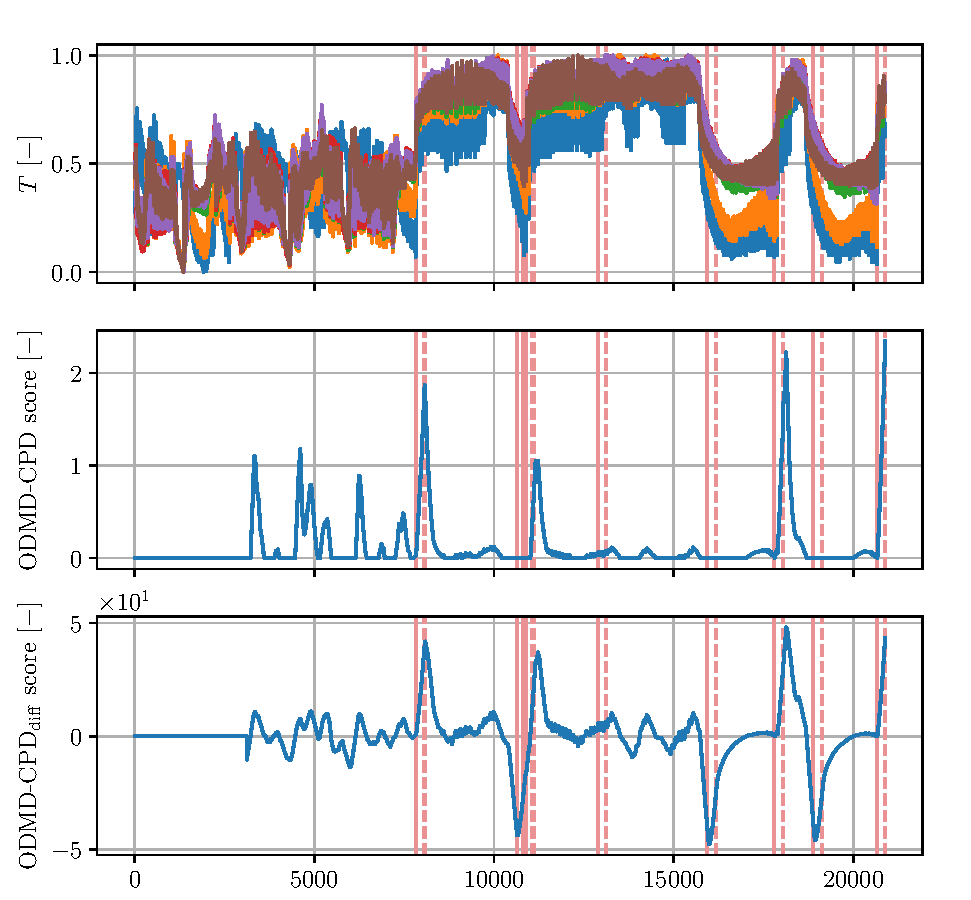
\includegraphics[width=\linewidth]{figures/bess-chd_p10-l2880_b240_t240roll_2880-dmd_w1.0-hx20.pdf}
    \caption{Faulty HVAC operation in BESS. Temperature profiles (top) show gradual elevation after the fault. The ODMD-CPD score (middle) detects the transition with early precursor signals. Error difference formulation (bottom) shows bidirectional detection (positive peaks for transitions to fault, negative for returns to normal).}
    \label{fig:bess}
\end{figure}

\section{Discussion}\label{sec:discussion}

\subsection{Comparison with State-of-the-Art}

Our ODMD-CPD framework offers distinct advantages over existing approaches:

\textbf{vs. Statistical methods (CUSUM, GLR):} Traditional statistical CPD methods~\cite{Ye2023} require knowledge of the data distribution and fail when temporal correlations exist. ODMD-CPD makes no distributional assumptions and explicitly models temporal dynamics through DMD modes.

\textbf{vs. Deep learning methods (autoencoders):} While methods like TIRE~\cite{DeRyck2021} achieve high accuracy, they lack interpretability and require extensive labeled data for training. ODMD-CPD provides physically interpretable detection statistics (reconstruction error ratios) and operates in a fully unsupervised manner. The DMD modes could reveal dominant frequencies and growth rates, enabling roost cause analysis.

\textbf{vs. Subspace methods (SSA, online SVD):} Methods like~\cite{Moskvina2003, Kawahara2007} detect changes in autonomous systems but do not account for sysntem dynamics and control inputs. ODMD-CPD explicitly disambiguates control effects from natural dynamics.

\textbf{vs. Kernel methods:} Non-parametric kernel approaches~\cite{Ferrari2023, Chu2022} work in arbitrary metric spaces but scale poorly with dimension (\(\mathcal{O}(n^2)\) vs. our \(\mathcal{O}(mr^2)\)) and provide less interpretable statistics.

\subsection{Applicability of ODMD-CPD}

The framework is particularly well-suited for:

\textbf{(1) Controlled systems:} Industrial processes where control actions significantly influence behavior. The DMDc formulation is essential here—standard DMD would misinterpret control as system changes.

\textbf{(2) Multi-scale dynamics:} Systems with multiple time constants (fast actuation, slow drift). Time-delay embedding \(h\) captures transients while windowed updates track long-term evolution.

\textbf{(3) Interpretability requirements:} Safety-critical applications where operators need to understand \textit{why} an alarm triggered. DMD modes reveal which frequencies changed, while \(Q_k\) quantifies relative severity.

\textbf{(4) Limited labeled data:} Existing installations where historical change-point annotations are unavailable. The unsupervised nature and online training enable immediate deployment.

\subsection{Practical Deployment Considerations}

Real-world deployment revealed several insights:

\textbf{Threshold selection:} While we used fixed \(\tau\) in experiments, adaptive thresholding based on historical \(Q_k\) distribution can reduce false alarms. A percentile-based approach (e.g., \(\tau = \text{95th percentile of }Q_k\) during normal operation) adapts to system-specific noise levels while may promote systematic bias.

\textbf{Multi-resolution detection:} Using multiple test windows \(c_1 < c_2 < \cdots\) enables detection at different time scales—fast \(c_1\) for abrupt changes, slow \(c_n\) for gradual drift. This addresses the "resolution-delay tradeoff" inherent in CPD.

\textbf{Feature attribution:} The reconstruction error can be decomposed by DMD mode: \(E = \sum_i E_i\) where \(E_i\) is the contribution of mode \(i\). This identifies \textit{which} dynamics changed.

\section{Conclusion}\label{sec:conclusion}

We presented an interpretable change-point detection framework (ODMD-CPD) based on truncated online Dynamic Mode Decomposition with control (toDMDc). By combining optimal rank truncation with online system identification, the framework maintains numerical stability while adapting to time-varying dynamics in real-time. The detection statistic, derived from reconstruction error ratios, provides interpretable measures of change severity with bounded detection delays while toDMDc tracks the linear interpretation of system dynamics.

Validation on three case studies—synthetic benchmarks, nonlinear controlled systems with delays, and industrial battery storage—demonstrates accurate detection across diverse change types (abrupt, gradual, drift) with low noise sensitivity. The method's computational efficiency (\(\mathcal{O}(mr^2)\) per update) and interpretability make it suitable for deployment in safety-critical industrial applications.


\bibliographystyle{IEEEtran}
\bibliography{main}

\end{document}
